\chapter{Results}

\section{General method of data processing}

The Helium spectrum from each measurement was saved to a text file, which included wavelengths with corresponding photon count. As an example of the Helium spectrum the unfiltered data with background noise, from a stationary measurement are shown in Fig. \ref{fig: demo data with noise}. 

\begin{figure}[h!]
\centering
\includegraphics[width=\linewidth]{figures/spectrum_with_noise_numbered.eps}
\caption{Example of the Helium spectrum from a measurement with the spectrograph, here illustrated by a spectrum from a stationary measurement. The six peaks that were used to determine the stability of the centroid wavelength value are marked and numbered one to six starting from the peak with the shortest wavelength.}
\label{fig: demo data with noise}
\end{figure}




The six emission lines used to determine the stability of the spectrograph for all three experiments, are marked and numbered from one to six in Fig. \ref{fig: demo data with noise} with the numbering starting from the peak with the shortest wavelength. The corresponding laboratory wavelength to peak number are shown in Tbl. \ref{tbl: Helium peaks}.
\begin{table}
\centering
    \begin{tabular}{cc}
    \hline
    Peak number & Wavelength [nm] \\ \hline
    1           & 388.86           \\
    2           & 447.14         \\
    3           & 501.58           \\
    4           & 587.56         \\
    5           & 667.82           \\
    6           & 706.52           \\ \hline
    \end{tabular}
    \caption{Wavelengths for the six spectral emission lines that were used in the experiments of this thesis \citep{helium-wavelength}.} 
    \label{tbl: Helium peaks}
\end{table}

The data from all measurements within each experiment firstly had the background noise from the CCD sensor removed. The background noise needed to be removed before is was possible to fit any functions to the data. This is done by using the intensity for wavelengths below 350 nm, where no spectral line are present from Helium, here only the noise on the CCD sensor is present, the average of the measured intensity for all wavelengths below \SI{350}{nm} was subtracted from the relative intensity for all data as the noise was uniform for the total wavelength range.
Then for every measurement the six marked peaks in Fig. \ref{fig: demo data with noise} will be found within each spectrum, and a Gaussian function will be fitted to each peak to determine the centroid wavelength of all the peaks. These wavelengths will be compared within all three experiments. Peak number 4, located around \SI{587}{nm}, was used in all three experiments to illustrate the data processing.

The general form of a Gaussian function is:
\begin{equation}
f(x) = A exp\left(-\frac{(x-b)^2}{2  \sigma^2}\right),
\label{eq: Single Gaussian}
\end{equation}
where, $A$ is the amplitude, $b$ is the centroid value of the peak and $\sigma$ is the standard deviation, which determines the width of the Gaussian profile.
\\
\\
The typical form of a peak with a fitted Gaussian function is shown in Fig. \ref{fig: double gauss}. It can be seen that the peak has a "shoulder" on the right which can be easily fit by two Gaussian. This is illustrated in Fig. \ref{fig: two single gauss}. %It is so because the peak is actually made up of two Gaussian functions that overlap, this is shown in fig. \ref{fig: two single gauss}, where the two single Gaussian functions that make up the combined Gaussian function, are illustrated separately. 
From section \ref{sec: Helium} it is known that the spectral lines of Helium are well defined. The distance between the two peaks was constant for all the lines in every measurements, which indicates that the "shoulder" of the spectral line is most like caused by internal reflections within the spectrograph. To determine the specific cause of this broadening, it would be necessary to take the spectrograph apart and do further testing. This is beyond the scope of this bachelor's thesis but the broadening will be filtered out in the data processing. 
\\
\\
To accurately identify the centroid of the peak, to be measured, it is necessary to fit to a combination of two Gaussian functions of the form:
\begin{equation}
f(x) = A_1 exp\left(-\frac{(x-b_1)^2}{2 \sigma_1^2}\right) + A_2 exp\left(-\frac{(x-b_2)^2}{2\sigma_2^2}\right),
\label{eq: Double Gaussian}
\end{equation}
and when a fit in the form of Eq. \ref{eq: Double Gaussian} has been found, we are able to get the information about the two separate Gaussian functions and thereby get the centroid information about the narrow and tall peak in which we are interested. 
\\
\\
One way to determine the uncertainty for every found wavelength is to use the \emph{Full Width at Half Maximum} (FWHM), which is the the width of the peak at half the maximum amplitude. FWHM is determined by the standard deviation, $\sigma$. The relationship between the two is given by:
\begin{equation}
FWHM = 2\sqrt{2ln2}\sigma,
\label{eq: FWHM}
\end{equation}
where $\sigma$ is obtained from the Gaussian function fitted to every peak.

\begin{figure}[h!]
    \centering
        \begin{subfigure}{0.5\textwidth}
        \centering
        \includegraphics[width=\linewidth]{figures/typisk_dobbelt_gauss.eps}
        \caption{Typical peak form, with double Gaussian fitted.}
        \label{fig: double gauss}
    \end{subfigure}%
    ~
    \begin{subfigure}{0.5\textwidth}
        \centering
        \includegraphics[width=\linewidth]{figures/to_enkelt_gauss.eps}
        \caption{The two single Gaussian functions that make up the fit in Fig. \ref{fig: double gauss}.}
        \label{fig: two single gauss}
    \end{subfigure}%
    \caption{Overview of the general observed Gaussian peak form. The left panel shows the form of the two combined Gaussian functions that are fitted to the experimental data and the right panel shows how the combined Gaussian can be split up into two single Gaussian functions. }
    \label{fig: Demo gauss peaks}
\end{figure}


Another way of determining the uncertainty is possible if an average of multiple measurements is done. Averaging multiple measurements is a practice often used when making observations from space. In space, observations are more prone to noise from radiation hitting the CCD sensor than on Earth, due to higher radiation in space. By stacking measurements, a single measurement with an increased value due to cosmic radiation hitting the CCD detector is less prominent and thereby reduces the uncertainty of the measured wavelength.
From $n$ measurements, the average, $\bar{x}$, and the standard deviation can be calculated from,

\begin{align}
\bar{x} = \frac{1}{n} \sum^{n}_{i=1}x_i,
\label{eq: avg}
\end{align}
\begin{align}
\sigma = \sqrt{\frac{1}{n-1} \sum_{i=1}^{n} (	x_i-\bar{x} )^2}.
\label{eq: std}
\end{align}
From the standard deviation the uncertainty, $S_{\bar{x} }$, of the average can be calculated,
\begin{align}
S_{\bar{x} } = \frac{\sigma}{\sqrt{n}} 
\label{eq: Sx}
\end{align}

\section{First Experiment - Stationary Measurements}

For the first experiment, code was written in \texttt{Matlab} to analyze all the measurements. In the data from every measurement the six peaks mentioned in Tbl. \ref{tbl: Helium peaks} were found. Each of the six peaks were then fitted to a function of the form seen in Eq. \ref{eq: Double Gaussian}. The parameters obtained from the fit were analyzed in order to identify which belonged to the narrow and taller peak. The parameters were analyzed by comparison of their amplitudes, and making sure that any fits with a negative amplitude were redone with limitations on the fitting parameters. Also the centroid parameters, which should have a constant distance to each other, were compared to make sure the fittings were done properly. With these parameters it was possible to fit a function of the form seen in Eq. \ref{eq: Single Gaussian}, to the data, where the measured noise from the earlier discussed "shoulder" Gaussian, was filtered out. The fit to a single Gaussian allowed for a more narrow width of the peak, which led to a smaller FWHM value and thereby a smaller uncertainty on the found wavelengths.
\\
\\
After the six emission peaks had been found in all measurements, outliers that had not been fitted properly by the code were removed from the data. Bad fittings were visible in the FWHM values. All the lines that had been fitted correctly had FWHM values around \SI{1}{nm}, while the badly fitted peaks had FWHM values above \SI{2}{nm}. The data filtered out by high FWHM values were less than \num{10}\% of the total measurements.
\\
\\
The measured wavelengths for each peak were then plotted against the time from the start of the experiment. For peak number 4, all the measured wavelengths are shown in Fig. \ref{fig: exp1 1000 maalinger} and the uncertainties in form of the FWHM for the measured wavelengths are shown in Fig. \ref{fig: exp1 1000 fwhm}. These are of the order of \SI{1}{nm}, when Eq. \ref{eq: FWHM} was used.


\begin{figure}[h!]
\centering
\begin{subfigure}{.9\textwidth}
\centering
\includegraphics[width = \linewidth]{stat_587_1000_maalinger.eps}
\caption{Measured wavelengths over time.}
\label{fig: exp1 1000 maalinger}
\end{subfigure}
\begin{subfigure}{.9\textwidth}
\centering
\includegraphics[width = \linewidth]{stat_587_fwhm.eps}
\caption{FWHM for wavelengths over time.}
\label{fig: exp1 1000 fwhm}
\end{subfigure}
\caption{In the top panel the measured wavelengths, for peak 4, from thousand measurements are shown over time. In the bottom panel the FWHM values for the wavelengths, for peak 4, are shown. }
\label{fig: Exp1 1000 samlet}
\end{figure}

The measurements were then binned to contain twenty measurements each and were analyzed using standard deviation described in Eq. \ref{eq: avg}, \ref{eq: std} and \ref{eq: Sx}. The average of each bin was calculated and the uncertainty was calculated from Eq. \ref{eq: Sx}. The measured wavelengths over time are shown in Fig. \ref{fig: exp1 bins} along with the calculated uncertainties.

The last processing of the data from the first experiment was done by taking the average of all the measured wavelengths for each peak. Then the uncertainty of the average for each peak was found. The average peak wavelengths are shown in Tbl. \ref{tbl: exp1 values} where they can be compared to the laboratory wavelengths of the peaks. The uncertainty for each emission line is shown in Fig. \ref{fig: exp1 usikkerhed peaks}.

\begin{figure}[!ht]
\centering
\begin{subfigure}{0.9\textwidth}
\centering
\includegraphics[width = \linewidth]{stat_587_bins_med_usikkerhed.eps}
\caption{Wavelengths measured when the measurements were binned.}
\label{fig: exp1 bins}
\end{subfigure}
~
\begin{subfigure}{0.9\textwidth}
\centering
\includegraphics[width = \linewidth]{stat_usikkerhed_alle.eps}
\caption{The uncertainty of the average wavelength for every peak.}
\label{fig: exp1 usikkerhed peaks}
\end{subfigure}
\caption{In the top panel the average wavelengths for bins containing twenty measurements are shown over time. The uncertainty of each wavelength is illustrated with errorbars. In the bottom panel the uncertainty of the total average wavelength measured for each peak is shown.}
\label{fig: exp1 samlet bins}
\end{figure}

\begin{table}
%\centering
\centerline{
    \begin{tabular}{ccccc}
    \hline
    Peak number & Average Wavelength [nm] & Laboratory Wavelength & $\Delta\lambda$ [nm]& $S_{\bar{x}}$ [$10^{-3}$ nm] \\ \hline
    1           & 389.02                  & 388.86      &    0.16      & 1.1                     \\
    2           & 447.22                  & 447.14       &    0.08     & 0.7                     \\
    3           & 501.56                  & 501.58        &    0.02    & 0.2                     \\
    4           & 587.46                  & 587.56         &    0.01   & 0.1                     \\
    5           & 667.66                  & 667.82         &    0.16   & 0.1                     \\
    6           & 706.34                  & 706.52          &    0.18  & 1.3                     \\ \hline
    \end{tabular}
    }
    \caption{Overview of the average wavelengths of the six peaks calculated from thousand measurements. The uncertainty of each average wavelength and the laboratory wavelengths are also shown.}
    \label{tbl: exp1 values}
\end{table}


\section{Second Experiment - Simulated Pointing via Vibrations}

For the second experiment the same methods were used to analyze the data from the measurements and to filter the measurements which were badly fitted. Based on the experience of determining the peak wavelengths from the measurements in the first experiment, both for every measurement and with measurements stacked, the wavelength was determined by binning measurements and calculating the uncertainty of the average wavelength. This is done because the uncertainty of the measured wavelengths when using every measurement alone is large compared to the range the found wavelengths are within.

The measurements were stacked to contain twenty data points each. The wavelength for the six peaks in every bin were calculated with Eq. \ref{eq: avg} and the uncertainties were calculated with Eq. \ref{eq: Sx}. For peak 4, the average wavelengths measured over time are shown in Fig. \ref{fig: exp2 bins}. 
\\
\\
For each peak of all the found wavelengths, were averaged and their uncertainties were calculated. The uncertainties are shown in Fig. \ref{fig: exp1 usikkerhed peaks}. The average wavelengths measured along with the calculated uncertainty for each peak are shown in Tbl. \ref{tbl: exp2 values}.

\begin{table}[h]
%\centering
\centerline{
    \begin{tabular}{ccccc}
    \hline
    Peak number & Average Wavelength [nm] & Laboratory Wavelength &$\Delta\lambda$ [nm]& $S_{\bar{x}}$ [nm] \\ \hline
    1           & 389.06                  & 388.86    &    0.20        & 0.01                     \\
    2           & 448.41                  & 447.14     &   1.27        & 0.37
                         \\
    3           & 503.29                  & 501.58     &    1.71   & 0.54
                         \\
    4           & 588.13                  & 587.56       &  0.57       & 0.47
                         \\
    5           & 667.82                  & 667.82         &   0    & 0.14
                         \\
    6           & 706.34                  & 706.52           &   0.18   & 0.02                     \\ \hline
    \end{tabular}
    }
    \caption{Overview of the average wavelengths of the six peaks calculated from thousand measurements.}
    \label{tbl: exp2 values}
\end{table}


\begin{figure}[!h]
\centering
\begin{subfigure}{0.8\textwidth}
\centering
\includegraphics[width = .7\linewidth]{vib_587_bins_med_usikkerhed.eps}
\caption{Wavelengths measured with bins containing twenty measurements for peak 4.}
\label{fig: exp2 bins}
\end{subfigure}
~
\begin{subfigure}{0.9\textwidth}
\centering
\includegraphics[width = .7\linewidth]{vib_usikkerhed_alle.eps}
\caption{The uncertainty of the average wavelength for every peak.}
\label{fig: exp2 usikkerhed peaks}
\end{subfigure}
\caption{In the top panel the calculated average wavelengths for peak 4, when stacking twenty measurements, are shown over time. The uncertainty of each wavelength is illustrated with errorbars and the mean over all the found wavelengths is shown. In the bottom panel the uncertainty of the total average wavelength found for each peak is shown.}
\label{fig: exp2 samlet bins}
\end{figure}

\newpage
\section{Third Experiment - Temperature Variations}

For the third experiment, 60 measurement were made for twelve different temperature steps. The temperatures are listen in Tbl. \ref{tbl: temp}.

\begin{table}[!h]
\centering
    \begin{tabular}{cccccc}
    \hline
    Step & Temperature [°C] & Step& Temperature [°C] & Step  & Temperature [°C] \\
    \hline
    1    & 19.5             & 5 & 32.4             & 9  & 42.2             \\
    2    & 25.0             & 6 & 35.9             & 10 & 44.8             \\
    3    & 28.1             & 7 & 36.9             & 11 & 47.8             \\
    4    & 29.9             & 8 & 39.8             & 12 & 49.3             \\
    \hline
    \end{tabular}
    \caption{The twelve temperature steps at which measurements were made for the third experiment.}
    \label{tbl: temp}
\end{table}


In the 60 measurements the six peaks were fitted in the same way as in the first and second experiment. The wavelengths measured for each peak in the 60 measurements were then used to calculate the average wavelength for every peak and their uncertainties were calculated. This was done for all temperatures. The measured shifts in wavelengths induced by the change in temperature for all six peaks are shown in Fig. \ref{fig: exp3 1_6}. 

\begin{figure}[!h]
\centering
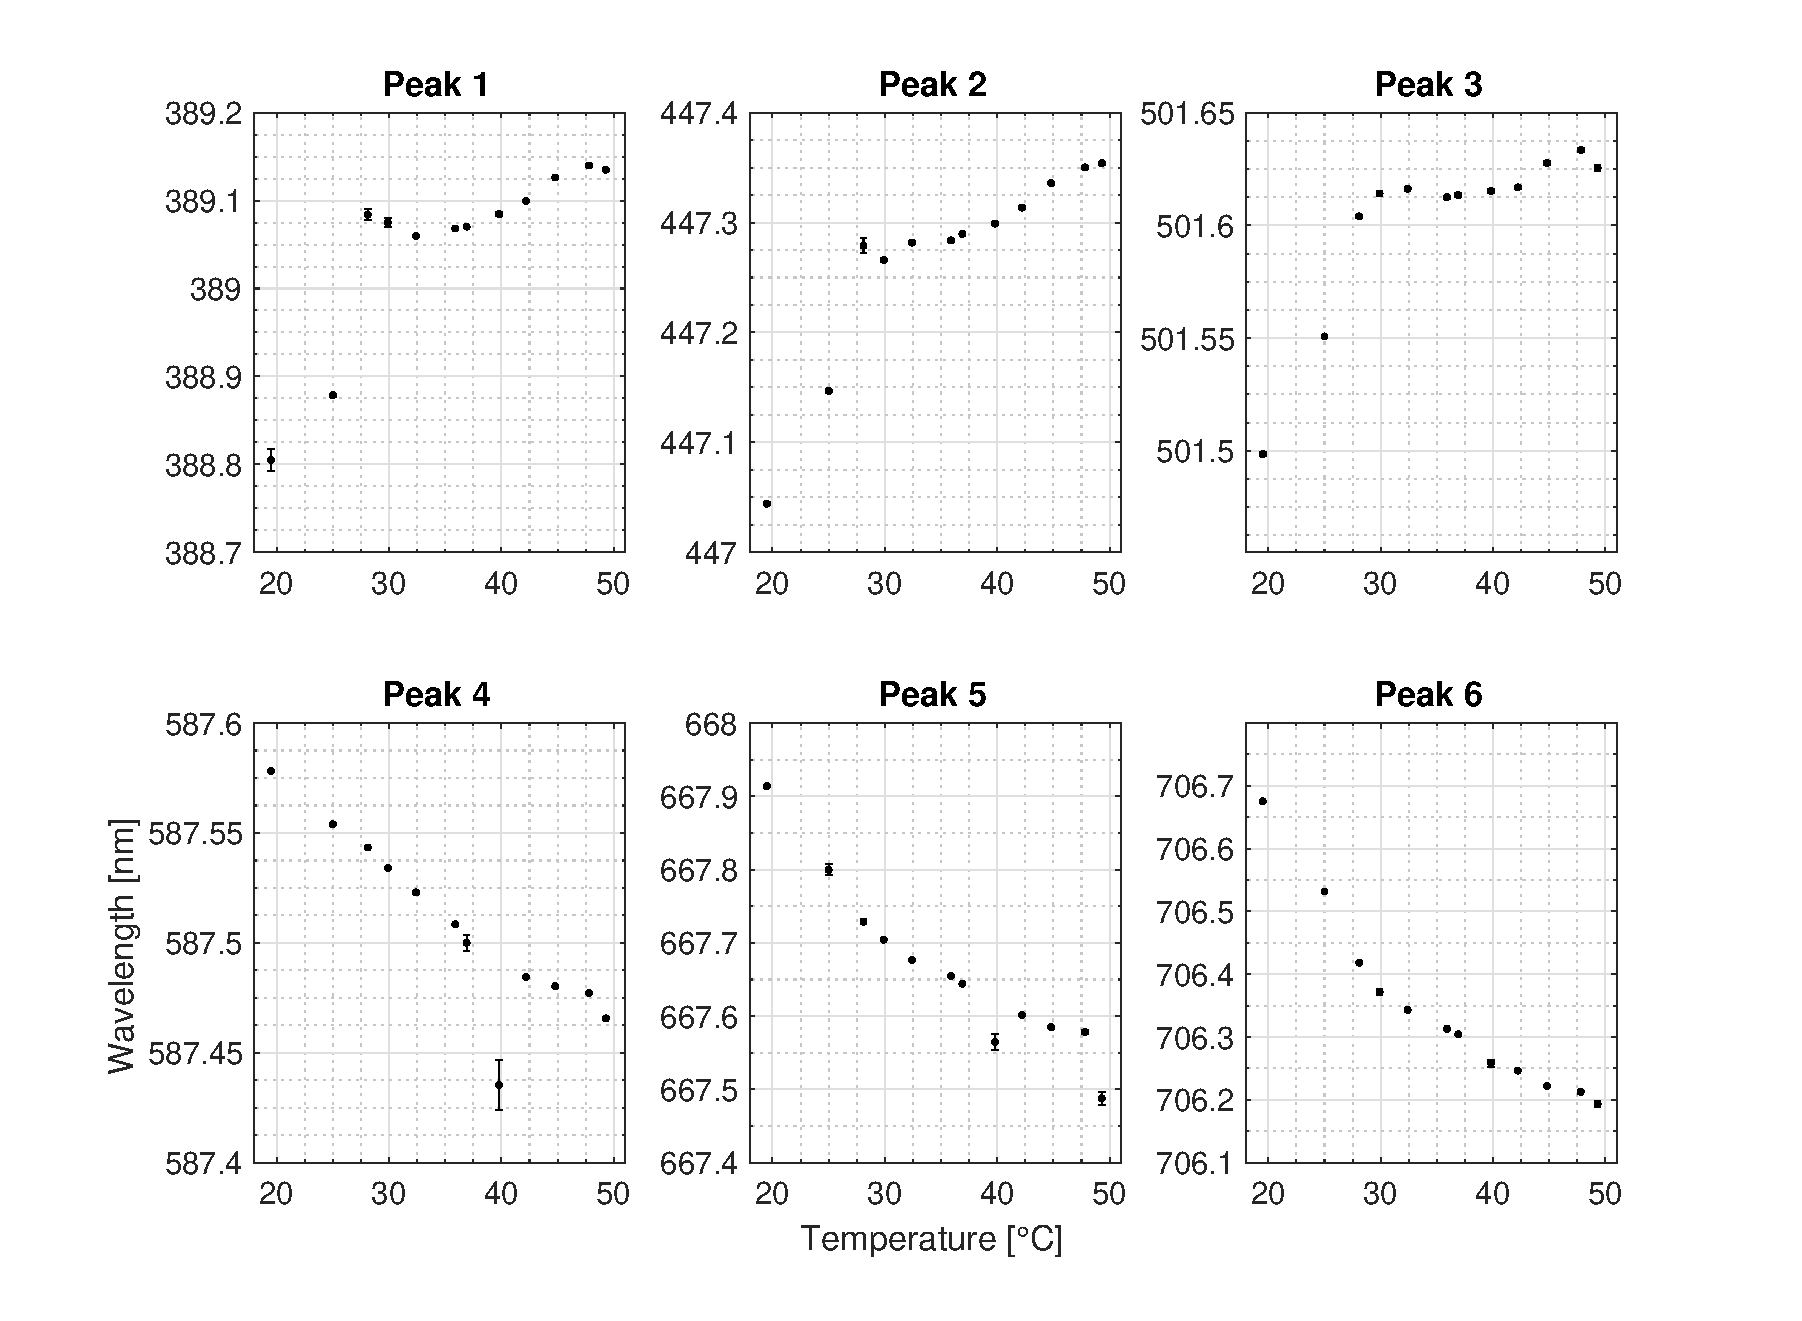
\includegraphics[width=\textwidth]{1_6_temp.eps}
\caption{The measured wavelengths by the spectrograph, for the six emission lines as a function of temperature. Uncertainties are calculated with Eq. \ref{eq: Sx}.}
\label{fig: exp3 1_6}
\end{figure}

Under the assumption, that the measured wavelengths of the peaks are shifted linearly as a function of temperature, the shift in wavelength for each peak  as a function of temperature was fitted to the function,
\begin{align}
\lambda_{shift}(T) = a_{shift} T + \lambda_{Laboratory}, 
\end{align}
where $\lambda_{shift}$ is the shifted wavelength value, $a_{shift}$ is the shift in wavelength per °C, $ T$ is the temperature and $\lambda_{Laboratory}$ is the the laboratory wavelength. The uncertainties, in form of the standard deviation, for the slope coefficients were found from their 95\%-confidence interval. 
\\
Based on the results in Fig. \ref{fig: exp3 1_6}, the slope coefficients, $a_{shift}$, for the six peaks were plotted against the wavelengths of the peaks. The slope coefficients as a function of wavelength were then fitted to the function,
\begin{align}
a_{shift}(\lambda) =  a_{slope} \lambda + b_{offset}, 
\label{eq: slope}
\end{align}
where $a_{slope}$ is the change of the $a_{shift}$ coefficients per wavelength, $\lambda$, and $b_{offset}$ is an offset.

The $a_{shift}$ coefficients as a function of wavelength are shown together with the fitted Eq. \ref{eq: slope} in Fig. \ref{fig: exp3 slope coeff.}.

\begin{figure}[!h]
\centering
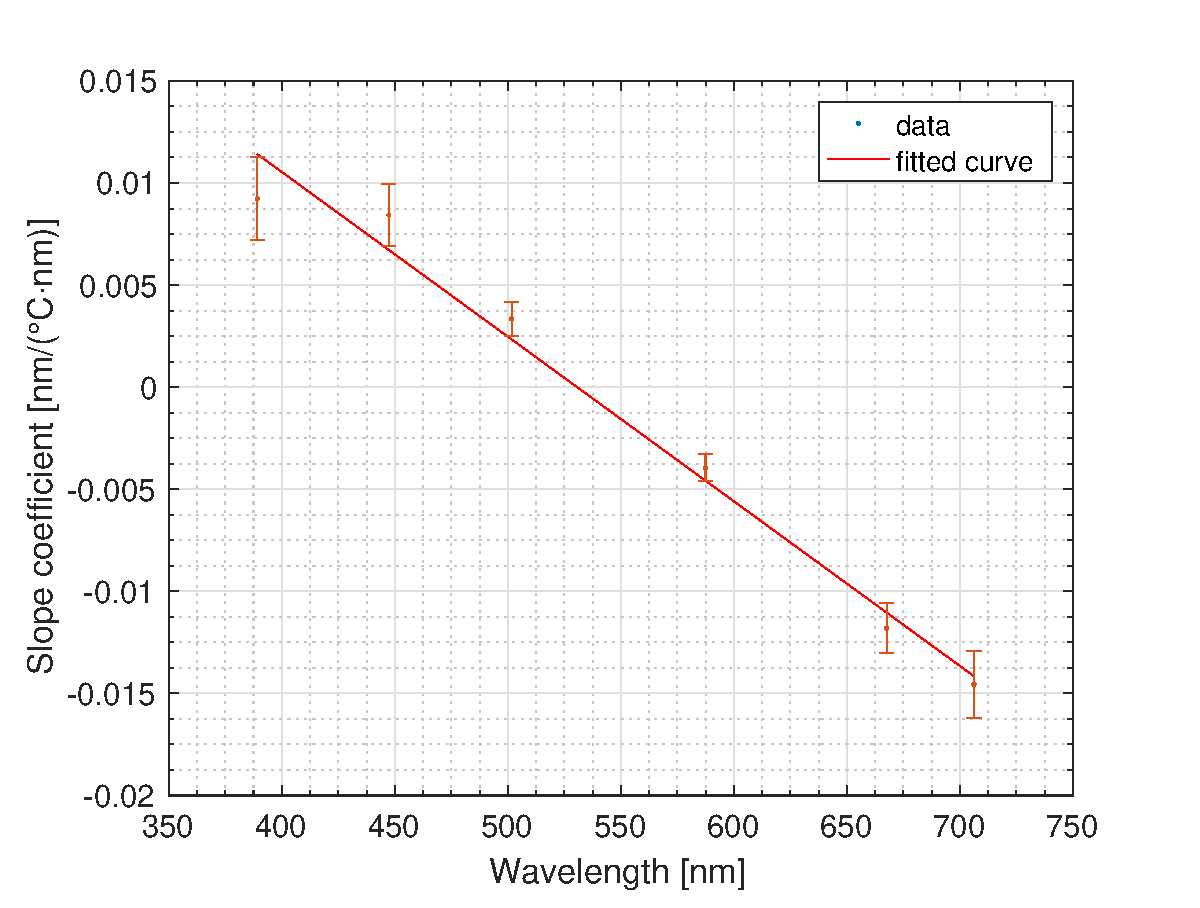
\includegraphics[width = \textwidth]{slope_function_of_wavelength.eps}
\caption{The $a_{shift}$ coefficients are shown as function of wavelength. The $a_{shift}$ coefficients are found by a linear fit to the measured wavelengths, for every emission line, under the assumption, that the found wavelengths of the peaks are shifted linearly as a function of temperature.}
\label{fig: exp3 slope coeff.}
\end{figure}

The results from the three experiments will be discussed in the following chapter.





